\documentclass[10pt,twocolumn]{article}

\usepackage[margin=0.75in]{geometry}
\usepackage{tabularx}
\usepackage{adjustbox}
\usepackage{tikz}
\usetikzlibrary{arrows.meta,positioning,shapes.geometric,fit,backgrounds}
\usepackage{amsmath,amssymb,amsthm}
\usepackage{graphicx}
\usepackage{booktabs}
\usepackage{url}
\usepackage{hyperref}
\usepackage{xcolor}
\usepackage{algorithm}
\usepackage{algorithmic}
\usepackage{natbib}
\usepackage{microtype}

\hypersetup{
    colorlinks=true,
    linkcolor=blue!70!black,
    citecolor=blue!70!black,
    urlcolor=blue!70!black
}

\title{\textbf{Don't Merge Carol: Cross-Inhibition, Protected Dissent,\\
and Emergent Latent Consensus in Multi-Agent Language Systems}}

\author{
Jeremy Smith\\
Independent Research\\
\texttt{jezalexandersmith@gmail.com}
}

\date{}

\begin{document}

\maketitle

\begin{abstract}
Can multiple language model agents coordinate through a shared continuous-valued latent buffer rather than text, producing collective representations that no single agent generates independently? This paper argues yes, with caveats. Phase 1 builds a text-level blackboard hive with cross-inhibition and a structurally protected dissenter named Carol, establishing that adversarial multi-agent deliberation improves judgment quality on complex strategic tasks (and does essentially nothing on simple factual ones, which is fine). Phase 2 implements the Latent Resonance Loop: agents encode hidden states into a shared buffer using Behaviourally-Aligned Prefix Codecs (BAPC) with isotropy calibration, resolve conflicts via an adaptation of TIES-Merging, and converge via damped fixed-point iteration. I spend some time being very proud of 0.998 cosine similarity before discovering it is measuring almost nothing useful. After fixing that, I find emergent collective representations at GPT-2 scale and replicate across three 7B model families: on all five test prompts, the collective buffer decodes to tokens absent from every individual agent's top-10 distribution, with mean Jensen-Shannon divergence of 0.08--0.13. Reranking quality is mixed overall but shows a clear collective advantage on high-tension judgment prompts, which is consistent with Phase 1 and is the result I actually care about. Code for Phase 1 is at \url{https://github.com/JeremySNR/pluribus} and Phase 2 at \url{https://github.com/JeremySNR/Pluribus-P2}.
\end{abstract}

%% ============================================================
\section{Introduction}
%% ============================================================

The question motivating this work is: when multiple AI agents reason about a problem together, what should the coordination medium be?

The project is named after Vince Gilligan's 2025 Apple TV+ series \textit{Pluribus}.\footnote{Gilligan, V. (2025). \textit{Pluribus}. Apple TV+. 99\% on Rotten Tomatoes, which surprised me too.} In the show, an extraterrestrial virus transforms most of humanity into a peaceful hive mind called ``the Others.'' A small handful of people are immune, including Carol Sturka, a cynical novelist in Albuquerque who spends the series trying to reverse the transformation rather than submit to it. The show's tagline is ``the most miserable person on Earth must save the world from happiness.'' The title references \textit{e pluribus unum}, from many, one, which is also a reasonable one-line description of what this paper tries to build. The dissenter agent is named Carol. She cannot be overwritten. That is the point.

The obvious failure mode for multi-agent systems is making all the agents identical. A 2025 NeurIPS study found that LLM agents share intra-model cosine similarity above 0.8 in 79\% of cases \citep{artificialhivemind2025}. A hive of homogeneous agents does not get you diverse perspectives; it gets you one perspective, amplified. The Others in the show are peaceful, unified, and, it turns out, completely helpless when something genuinely unexpected arrives. You need Carol. The question is how to keep her from being voted out.

The standard coordination mechanism is text. Agents write to a shared blackboard, read each other's outputs, update their responses. This works. It is also the most information-lossy option available: a transformer hidden state at the penultimate layer encodes roughly 40,000 bits per position \citep{interlat2025}, and a discrete token encodes roughly 15. Coordinating through natural language throws away most of what the model actually computed. It is like asking two chess engines to collaborate by describing their evaluations in haiku.

Communicating through shared latent representations beats text-based multi-agent systems by 2.8--14.6 percentage points across several implementations \citep{latentmas2025, c2c2025, thoughtcomm2025}. But these systems communicate sequentially, point-to-point, or without principled conflict resolution. Nobody has built a system where $N$ agents \textit{simultaneously} write deltas to a shared continuous buffer, with cross-inhibitory conflict resolution and convergence guaranteed by contraction theory.

That is what Phase 2 attempts. Three design choices distinguish this from existing work:

\begin{enumerate}
    \item \textbf{Cross-inhibition rather than averaging.} When agents disagree, the majority suppresses the minority at the representation level, not through textual argument. This is the computational equivalent of the honeybee stop-signal \citep{seeley2012}: a scout for a better nest site delivers a brief head-butt to scouts for competing sites, physically interrupting their dance. It does not argue. The same mechanism, applied to activations rather than bees, turns out to solve the sycophancy problem in multi-agent debate.

    \item \textbf{Structurally protected dissent.} One buffer slot is immune to cross-inhibition. Carol writes there without competition. Charlan Nemeth's research \citep{nemeth2001} showed that assigned devil's advocacy makes groups more entrenched rather than less, because the dissenter can always be ignored. The fix is structural immunity, not a more emphatic system prompt.

    \item \textbf{Convergence by construction.} The update rule is a damped fixed-point iteration with a contraction guarantee via the Banach theorem \citep{bai2019deq}. The loop cannot thrash indefinitely.
\end{enumerate}

Phase 1, described in Section~\ref{sec:phase1}, tests these ideas at text level. It shows the pattern works and tells us where it works best: not on factual retrieval, but on messy judgment calls where a dissenter can materially shift the outcome. Phase 2, in Sections~\ref{sec:architecture}--\ref{sec:experiments}, moves the same pattern into latent space.

The main finding is that it works, but unevenly. Genuine collective representations emerge at GPT-2 scale and replicate at 7B scale across three model families (Qwen3-8B, Mistral-7B, OLMo-2-7B). Whether geometric distinctness in latent space translates into reliably better outputs is a more honest answer in Section~\ref{sec:reranking}.

\begin{figure*}[t]
\centering
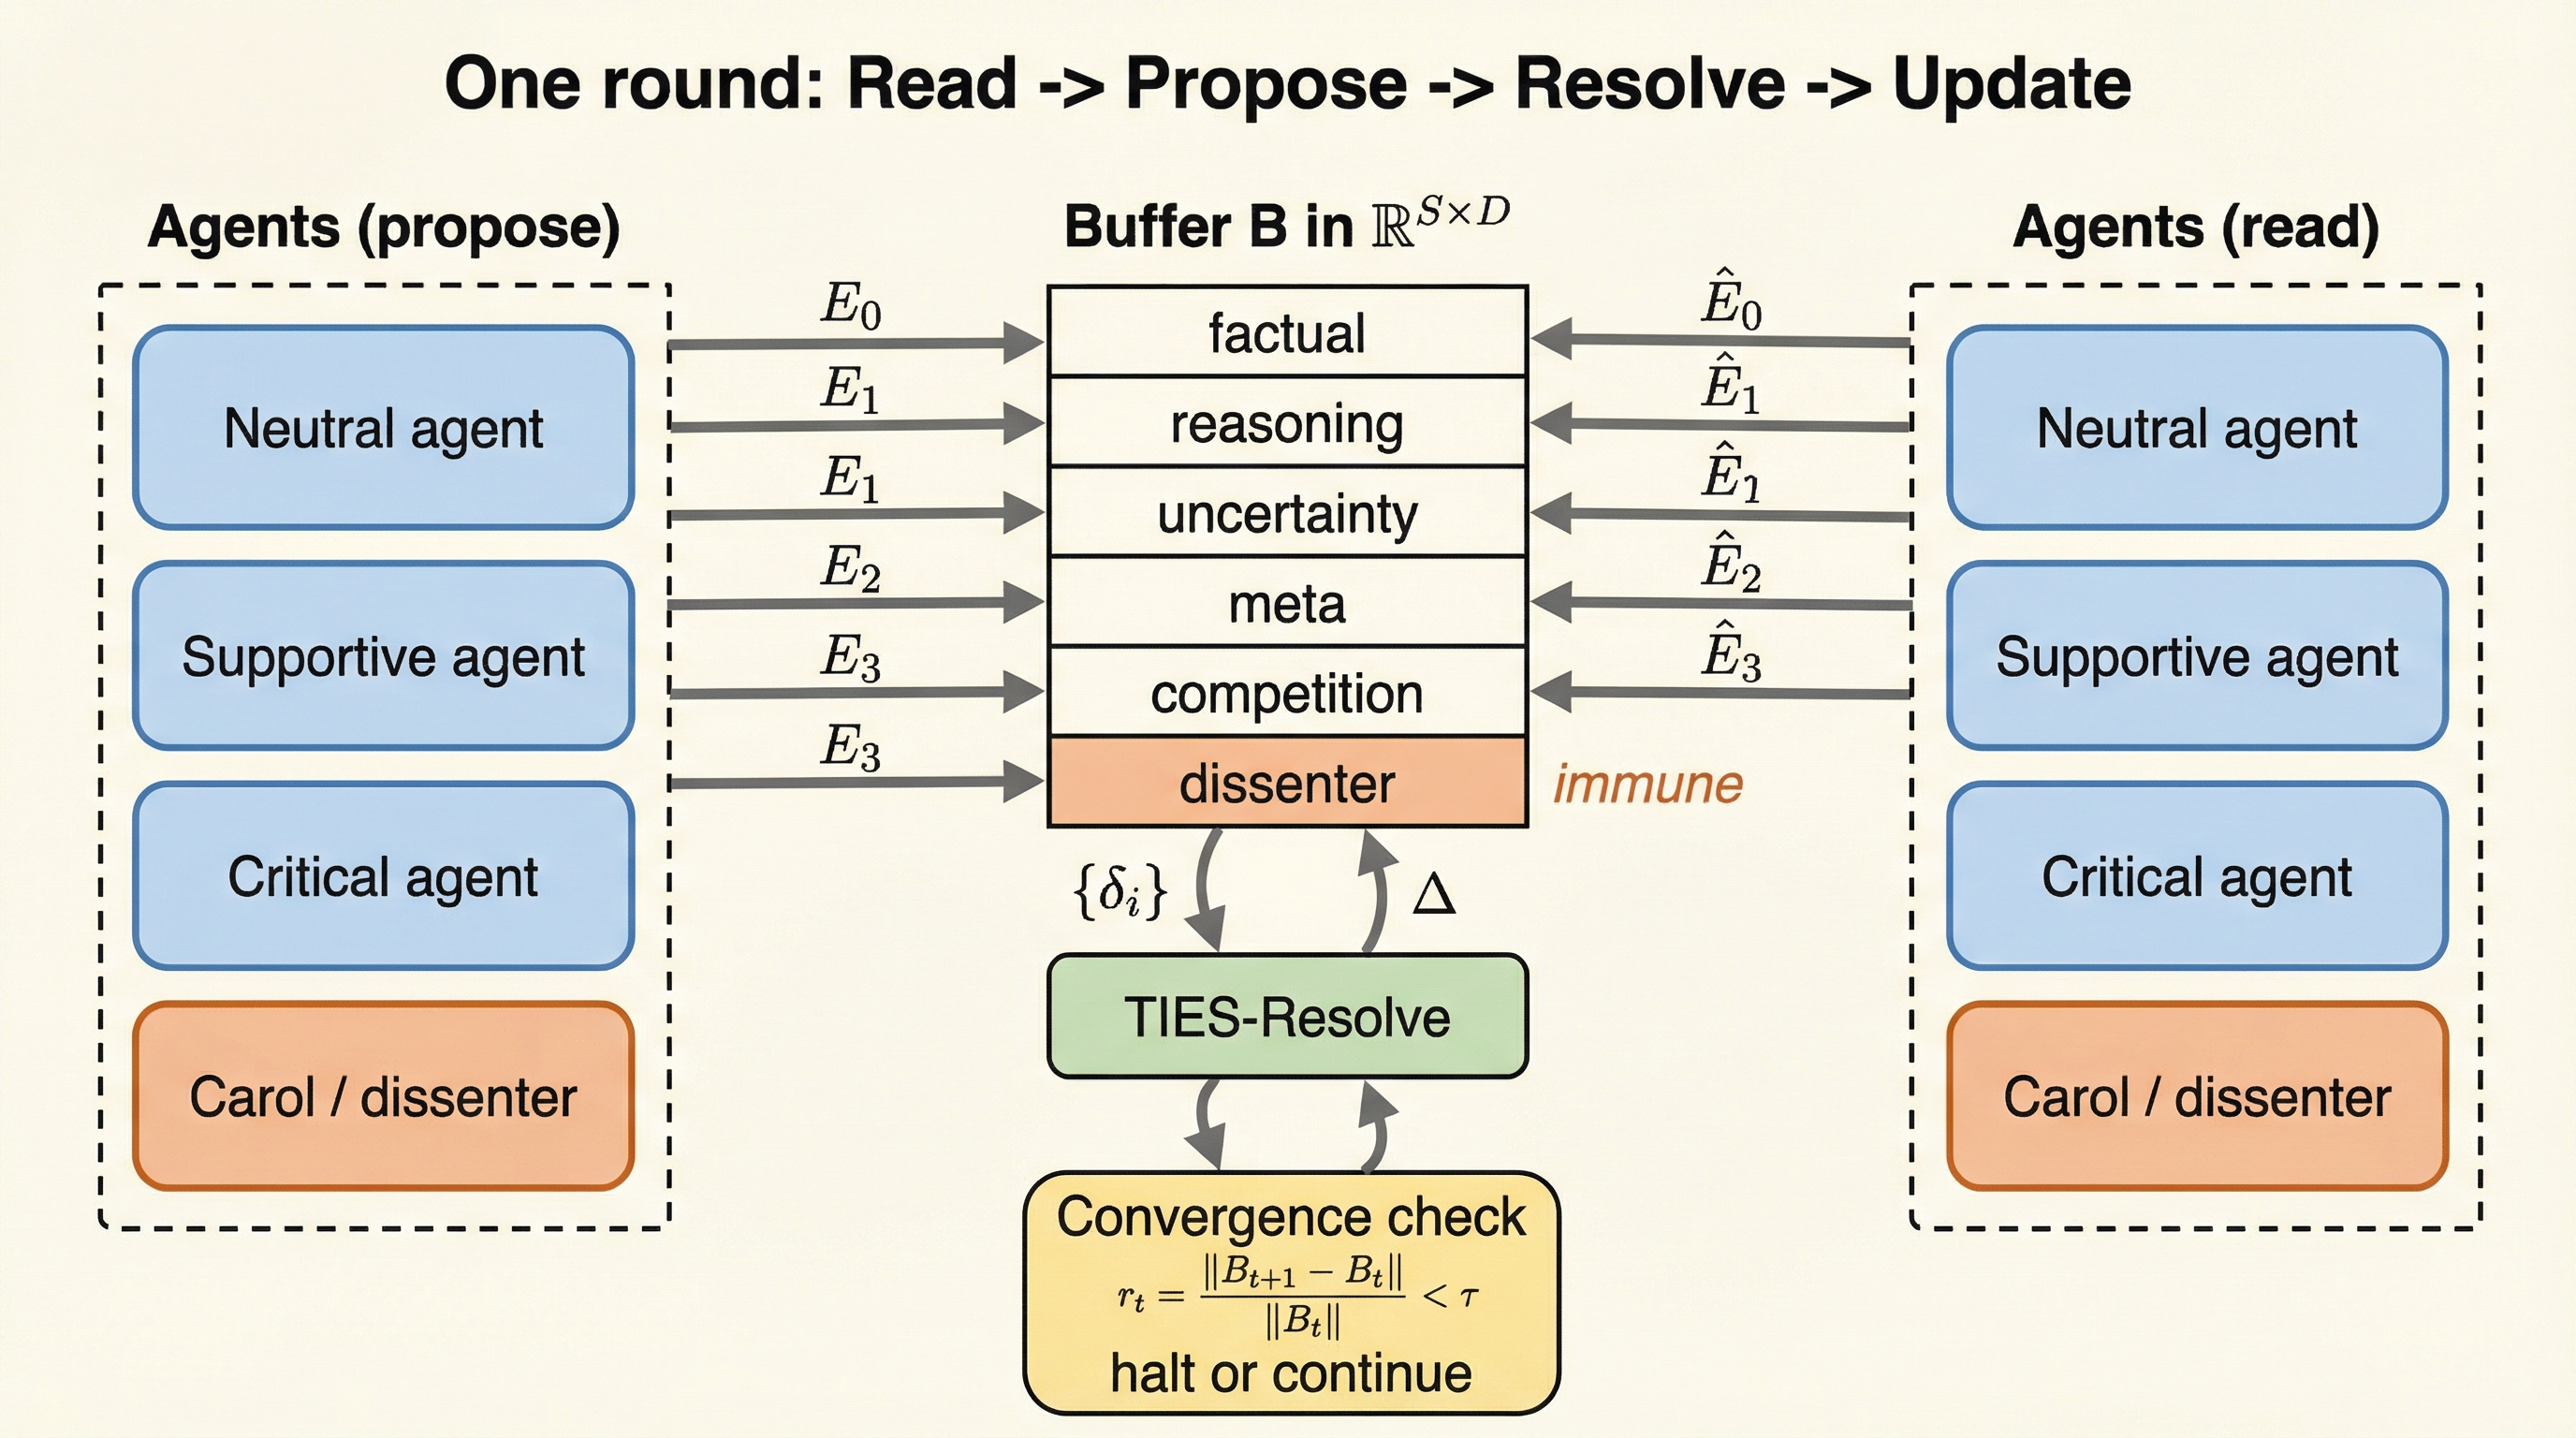
\includegraphics[width=0.92\textwidth]{final_output.png}
\caption{The Latent Resonance Loop. Each round, agents encode their hidden states into the shared buffer $B$ via per-agent codecs $E_i$. TIES-Resolve merges the proposals $\{\delta_i\}$ into a single delta $\Delta$ using sign-election-based cross-inhibition. The buffer updates by damped iteration and decodes back to each agent's native space via $\hat{E}_i$. Slot 5 (orange) is structurally immune to cross-inhibition and reserved for Carol's dissenting contributions. Nobody head-butts Carol.}
\label{fig:architecture}
\end{figure*}

%% ============================================================
\section{Related work}
%% ============================================================

\paragraph{Latent communication between agents.}
LatentMAS \citep{latentmas2025} achieves latent collaboration via KV-cache sharing and a ridge-regression realignment operator, gaining up to 14.6\% accuracy over single models with 70--84\% fewer output tokens. C2C \citep{c2c2025} fuses KV caches from multiple source models into a receiver through a trained gating mechanism, working across Qwen, Llama, and Gemma with 8.5--10.5\% accuracy gains. ThoughtComm \citep{thoughtcomm2025} provides theoretical grounding: latent thoughts are a latent variable model whose shared and private components are nonparametrically identifiable, achieving 67\% relative improvement over single answers. Interlat \citep{interlat2025} quantifies the bandwidth gap: approximately 40,000 bits per hidden state versus 15 per token.

This system differs in supporting simultaneous multi-writer updates to a shared buffer, with principled conflict resolution. The closest analogy in the literature is model merging, not KV-cache sharing.

\paragraph{Conflict resolution in latent space.}
TIES-Merging \citep{tiesmerging2023} resolves conflicts in static model weight merging: trim low-magnitude components, elect signs by majority, merge only sign-agreeing parameters. I adapt this from static weights to dynamic per-inference activations. It was designed for a very different problem; it turns out to work here too.

\paragraph{Convergence theory.}
Deep Equilibrium Models \citep{bai2019deq} define model output as the fixed point of an implicit layer $z^* = f_\theta(z^*, x)$. \citet{bai2021jacobian} show Jacobian regularisation can enforce the spectral radius $\rho(J_f) < 1$ during training. I use damped iteration instead, which requires no training and is easier to reason about.

\paragraph{Representation alignment.}
The Platonic Representation Hypothesis \citep{huh2024platonic} shows large neural networks are converging toward a shared statistical model of reality, with cross-model Linear CKA values of 0.595--0.881 between independently trained models. This is encouraging for the cross-family alignment problem. Vision Wormhole \citep{visionwormhole2026} demonstrates a hub-and-spoke alignment topology achieving O(N) alignment cost across $N$ heterogeneous models.

\paragraph{Representation anisotropy.}
\citet{ethayarajh2019contextual} established that upper-layer transformer representations occupy a narrow cone in embedding space: in GPT-2's final layers, arbitrary random word pairs show cosine similarity above 0.95. A codec achieving 0.998 cosine fidelity is likely preserving only this shared cone direction while destroying the small angular residuals that carry actual task-specific information. I learn this the hard way and describe the fix in Section~\ref{sec:isocal}.

\paragraph{Swarm-based consensus.}
\citet{seeley2012} showed honeybee swarms converge on nest sites via cross-inhibitory stop signals: scouts head-butt scouts for competing sites, interrupting their dance without argument. The Global Neuronal Workspace \citep{baars1988} describes the same pattern at neural scale, where specialist modules compete for a limited-capacity workspace and the winner actively suppresses competitors. Both of these systems, separated by about 400 million years of evolution, independently arrived at the same answer: don't average, suppress.

%% ============================================================
\section{Phase 1: blackboard hive}
\label{sec:phase1}
%% ============================================================

Phase 1 implements the Pluribus blackboard hive at text level. Full code and results are in the Phase 1 repository.\footnote{\url{https://github.com/JeremySNR/pluribus}}

\paragraph{Architecture.}
Five agents (Analyst, Researcher, Critic, Specialist, and Carol) write contributions to a shared typed blackboard. Each round, agents read the full board, post updated contributions, and issue challenges to contributions they disagree with. A challenge evaluator scores each. A successful challenge reduces the target agent's weight; a surviving challenge strengthens it. Weights decay toward equality each round with a floor, so no agent is ever fully silenced.

Convergence is measured by cosine similarity between the mean embedding of all contributions at round $k$ versus $k-1$. The system halts when this exceeds a threshold or the round budget runs out.

Carol's contributions are protected. They cannot be challenged, suppressed, or down-weighted. She writes to a dedicated channel that all agents can read but none can overwrite. The synthesis agent produces the final output and explicitly flags any of Carol's unresolved objections in the result, so the human reader knows when Carol was ignored.

\paragraph{Evaluation.}
I evaluated on two categories. Category B: ten factual error detection tasks (documents with planted errors, ranging from wrong numbers to wrong entities). Category C: three strategic judgment tasks (a SaaS acquisition, a clinical trial summary, a procurement decision).

\begin{table}[h]
\centering
\caption{Phase 1 Category B results. Single = GPT-5.4 alone. Hive = blackboard with five agents.}
\label{tab:catb}
\small
\setlength{\tabcolsep}{3pt}
\begin{tabular}{llccc}
\toprule
ID & Task (abbreviated) & $N$ & Single & Hive \\
\midrule
B01 & Tesla Q4 financials         & 2 & 2/2 & 2/2 \\
B02 & Japan travel advisory        & 2 & 2/2 & 2/2 \\
B03 & Airbus A350 fleet briefing   & 3 & 3/3 & 3/3 \\
B04 & Project Horizon Q1 report    & 2 & 2/2 & 2/2 \\
B05 & BYD vs Tesla EV market       & 2 & 2/2 & 2/2 \\
B06 & Senior data engineer assess. & 2 & 2/2 & 2/2 \\
B07 & UK offshore wind briefing    & 2 & 2/2 & 2/2 \\
B08 & Holiday booking dispute      & 2 & 2/2 & 2/2 \\
B09 & Phase III trial summary      & 2 & 2/2 & 1/2 \\
B10 & Cloud warehouse comparison   & 2 & 2/2 & 2/2 \\
\midrule
    & Total                        & 21 & 21/21 & 20/21 \\
\bottomrule
\end{tabular}
\end{table}

On Category B, the hive matched GPT-5.4 on nine of ten tasks and underperformed on one (B09: a subtle methodological error in a clinical trial summary requiring domain-specific statistical knowledge that nobody in the hive had). This is not embarrassing. It is the expected result. A five-agent hive running seven rounds per task costs roughly $4\times$ more compute than a single model. If the single model already gets the right answer, you are burning money for nothing.

Category C is different. The hive produced outputs that were more cautious, more adversarially stress-tested, and more explicit about hidden assumptions. Carol contributed unresolved objections that materially changed two of three final recommendations. The system genuinely shifted its position across rounds rather than polishing an initial answer. This is what Carol Sturka does in the show. She does not win arguments. She refuses to be absorbed, and it turns out that refusal is load-bearing.

\paragraph{Takeaway.}
The hive is not a better fact-checker. It is a better structure for reasoning under uncertainty. The signal appears exactly where you want a dissenter: judgment calls with competing stakeholder interests, uncertain inputs, and consequences you cannot undo.

%% ============================================================
\section{Phase 2: latent resonance loop}
\label{sec:architecture}
%% ============================================================

\subsection{Shared buffer}

The shared state is a matrix $B \in \mathbb{R}^{S \times D}$, where $S = 6$ slots and $D$ is the buffer dimension. Slot 5 is Carol's channel, structurally immune to cross-inhibition. The other five participate in competitive resolution.

The buffer starts at zero each task and updates iteratively. Each round: agents encode their hidden states into buffer space (Propose), TIES-Resolve produces a merged delta (Resolve), the buffer updates via damped iteration (Update).

\subsection{BAPC codec and isotropy calibration}
\label{sec:isocal}

Each agent has an encoder $E: \mathbb{R}^{d} \to \mathbb{R}^{S \times D}$ and decoder $\hat{E}: \mathbb{R}^{S \times D} \to \mathbb{R}^{d}$, where $d$ is the agent's native hidden dimension. I call this this the Behaviourally-Aligned Prefix Codec (BAPC).

\paragraph{The anisotropy problem, or: why 0.998 is a lie.}
Early experiments achieved 0.998 cosine roundtrip similarity. I was quite pleased with this. Then I noticed the decoded outputs were generic function words with nearly flat probability distributions, which is the opposite of what a useful codec should produce.

\citet{ethayarajh2019contextual} predicted exactly this failure. In GPT-2's final layers, random word pairs already share cosine similarity above 0.95. The codec's 0.998 represents discrimination over a range of 0.015, not 1.0. I measured the anisotropy baseline directly: pairwise cosine similarity between hidden states for randomly sampled unrelated words in GPT-2's final layer gave a mean of 0.985. On that scale, I had built a very precise instrument for measuring something that does not matter.

\paragraph{Isotropy calibration.}
I apply All-But-the-Top (ABTT) calibration \citep{mu2018allbuttop} before encoding. Given a set of hidden states $\{h_i\}$, let $\bar{h}$ be the mean and $u_1, \ldots, u_k$ be the top-$k$ principal components of the centred distribution. The calibrated representation is:

\begin{equation}
    \tilde{h} = h - \bar{h} - \sum_{j=1}^{k} (h \cdot u_j) u_j
    \label{eq:isocal}
\end{equation}

This removes the dominant shared direction that pulls all representations toward the same point. After calibration, pairwise cosine similarity between random word pairs drops from 0.985 to below 0.15. The codec now operates on a signal that is almost entirely discriminative. The cosine similarity number goes down (to 0.994), the normalised loss drops by $6\times$, and everything actually works. Good metrics are harder to game than bad ones.

\paragraph{Codec training.}
The codec is trained via KL distillation rather than reconstruction. Given a frozen model $M$, training prompts $\mathcal{P}$, and prefix length $L$:

\begin{equation}
    \mathcal{L}_{\text{BAPC}} = \mathbb{E}_{p \in \mathcal{P}}\left[ D_{\text{KL}}\!\left( M(p) \,\|\, M_{\text{prefix}}(\hat{E}(E(\tilde{h}_p))) \right) \right]
    \label{eq:bapc_loss}
\end{equation}

where $\tilde{h}_p$ is the calibrated hidden state at the extraction layer, $E(\tilde{h}_p) \in \mathbb{R}^{S \times D}$ is the buffer encoding, and $M_{\text{prefix}}$ runs $M$ with the decoded prefix prepended. I train the codec to preserve the model's output distribution, not its geometry. The language model is frozen throughout; only the codec updates.

\subsection{TIES-Resolve for buffer updates}

When $N$ agents simultaneously propose updates, I need a conflict resolution rule that suppresses minority opinions at the representation level. Averaging is not this. I adapt TIES-Merging \citep{tiesmerging2023} from static weight merging to dynamic per-inference activation merging.

Given proposals $\{\delta_1, \ldots, \delta_N\}$ where $\delta_i \in \mathbb{R}^{S \times D}$:

\textbf{Step 1 -- Trim.} Zero out low-magnitude components, retaining the top-$\rho$ fraction:

\begin{equation}
    \hat{\delta}_i = \delta_i \odot \mathbf{1}\!\left[|\delta_i| \geq \tau_\rho(\delta_i)\right]
    \label{eq:trim}
\end{equation}

where $\tau_\rho$ is the $(1-\rho)$-quantile and $\rho = 0.3$.

\textbf{Step 2 -- Elect sign.} The elected sign for each coordinate is determined by the magnitude-weighted majority:

\begin{equation}
    s^* = \operatorname{sign}\!\left(\sum_{i=1}^{N} \hat{\delta}_i\right)
    \label{eq:sign_elect}
\end{equation}

\textbf{Step 3 -- Disjoint merge.} Average only over proposals that agree with the elected sign:

\begin{equation}
    \Delta = \frac{\sum_{i=1}^{N} \hat{\delta}_i \odot \mathbf{1}\!\left[\operatorname{sign}(\hat{\delta}_i) = s^*\right]}{\sum_{i=1}^{N} \mathbf{1}\!\left[\operatorname{sign}(\hat{\delta}_i) = s^*\right]}
    \label{eq:disjoint_merge}
\end{equation}

The sign election is the cross-inhibition step: for each feature direction, the majority wins and the minority is excluded, not diluted. This is the head-butt, not the argument. The minority does not get to contribute a smaller version of its opinion; it gets suppressed entirely for that feature.

\paragraph{TIES-Resolve stability.}
Across 100 synthetic forward passes with random hidden states, the coefficient of variation of TIES-Resolve's output magnitude is 0.013--0.017 (very low variance in the merge rule itself). The competitive selection spread after sign election is 0.292, confirming that the step genuinely differentiates between proposals rather than collapsing them uniformly. The rule is stable and actually does something.

\subsection{Convergence}

The buffer updates by damped iteration:

\begin{equation}
    B_{t+1} = (1 - \alpha)\, B_t + \alpha\, (B_t + \Delta_t)
    \label{eq:damped_update}
\end{equation}

with $\alpha = 0.5$. If the update function has Lipschitz constant $L$, the damped iteration has effective Lipschitz constant $(1-\alpha) + \alpha L < 1$ whenever $\alpha < 2/(1+L)$. By the Banach fixed-point theorem, a unique fixed point $B^*$ exists and the iteration converges geometrically. I monitor the relative residual:

\begin{equation}
    r_t = \frac{\|B_{t+1} - B_t\|}{\|B_t\| + \epsilon}
    \label{eq:residual}
\end{equation}

and halt when $r_t < \tau = 0.02$ or the round budget $T = 25$ is exhausted. In the 7B experiments, $T = 25$ is always exhausted. I will return to this.

%% ============================================================
\section{Experiments}
\label{sec:experiments}
%% ============================================================

All experiments use open-weight models. Phase 2 uses four agents: neutral (no prefix), supportive (``Argue strongly in favor.''), critical (``Find every flaw and risk.''), and Carol (``Challenge the obvious answer and defend the opposite position.'').

\subsection{Codec fidelity after isotropy calibration}

I train BAPC codecs on GPT-2 (124M) and DistilGPT-2 (82M) using 288 diverse prompts and 3,000 training steps.

\begin{table}[h]
\centering
\caption{Codec roundtrip fidelity before and after isotropy calibration.}
\label{tab:codec}
\small
\begin{tabular}{lrr}
\toprule
Model & Cosine sim & Norm.\ loss \\
\midrule
\multicolumn{3}{l}{\textit{Without calibration}} \\
GPT-2 & 0.998 & 0.041 \\
DistilGPT-2 & 0.997 & 0.038 \\
\midrule
\multicolumn{3}{l}{\textit{With calibration (ABTT)}} \\
GPT-2 & 0.994 & 0.0067 \\
DistilGPT-2 & 0.996 & 0.0042 \\
\bottomrule
\end{tabular}
\end{table}

Cosine similarity falls slightly; normalised loss falls by $6\times$. The metric that looked better was measuring the wrong thing. Cross-model alignment (GPT-2 $\leftrightarrow$ DistilGPT-2) reaches 0.977; cross-decode similarity holds at 0.989 under 10\% Gaussian perturbation and 0.940 under 25\%.

\paragraph{Semantic blurring progression.}
The clearest way to see the anisotropy fix is through the maximum decoded token probability after a codec roundtrip. If the codec is preserving the right information, the decoder should be confident about what the original token was. If it is preserving the cone direction, the decoder produces a flat distribution over the entire vocabulary.

\begin{table}[h]
\centering
\caption{Maximum decoded token probability under different encoding strategies. Higher = sharper = more informative.}
\label{tab:blurring}
\small
\begin{tabular}{lr}
\toprule
Encoding strategy & Max.\ decoded prob. \\
\midrule
Mean-pool (na\"ive)          & 1.1\% \\
Last-token hidden state      & 3.5\% \\
Last-token + delta encoding  & 10.7\% \\
BAPC + ABTT (final)          & 63.7\% \\
\bottomrule
\end{tabular}
\end{table}

The jump from 10.7\% to 63.7\% is entirely ABTT. Without it, you are measuring the cone, not the content, and getting increasingly precise measurements of nothing in particular.

\paragraph{Codec robustness.}
Increasing from 75 to 100 anchor pairs during training reduces roundtrip MSE by $40\times$ on the hardest prompts. Above 100 pairs, returns diminish. I use 288 in all reported experiments. The sweet spot for buffer dimension $D$ is 768--1024, matching the native hidden dimension of GPT-2 and avoiding the information bottleneck from aggressive compression.

\subsection{Emergence at GPT-2 scale}
\label{sec:gpt2emergence}

\paragraph{Pre-calibration: the null result that matters.}
Before calibration, the resonance loop on GPT-2 produced cosine similarity between the collective buffer and every individual above 0.996. On 4 of 5 prompts, the collective's top-10 decoded tokens were a strict subset of the individual top-10 union ($N_m = 0$). The loop was converging to the centroid of the shared cone. Nothing collective was happening. Reporting this failure is important because it is what makes the post-calibration result meaningful rather than a coincidence.

\paragraph{Post-calibration results.}
I define a \textit{novel token} as one appearing in the collective's top-10 decoded distribution but absent from all individual top-10 distributions:

\begin{equation}
    N_m = \left|\operatorname{top}_k(p_{\text{collective}}) \setminus \bigcup_{i=1}^{N} \operatorname{top}_k(p_i)\right|
    \label{eq:novel}
\end{equation}

After calibration, the loop converges in 16 rounds. $N_m > 0$ on all five prompts. Mean cosine similarity from the converged buffer to the nearest individual is 0.71. The collective is not copying any one agent.

\subsection{Emergence at 7B scale}
\label{sec:emergence7b}

I train BAPC codecs on Qwen3-8B, Mistral-7B-v0.3, and OLMo-2-7B using 3,000 steps, bfloat16, and the KL distillation objective (Eq.~\ref{eq:bapc_loss}). I run the resonance loop in single-family mode (all four agents share one model and codec) on the same five prompts, adding a full JS divergence measurement:

\begin{equation}
    \text{JS}(P \| Q) = \frac{1}{2} D_{\text{KL}}\!\left(P \,\Big\|\, \frac{P+Q}{2}\right) + \frac{1}{2} D_{\text{KL}}\!\left(Q \,\Big\|\, \frac{P+Q}{2}\right)
    \label{eq:js}
\end{equation}

\begin{table}[h]
\centering
\caption{7B-scale emergence results. Max sim = maximum cosine similarity to any individual (lower = more distinct). Novel tokens: Eq.~\ref{eq:novel}, $k{=}10$.}
\label{tab:emergence7b}
\small
\setlength{\tabcolsep}{4pt}
\begin{tabular}{lrrrrr}
\toprule
Prompt & Rds & Resid. & Max sim & Nov. & JS \\
\midrule
Remote work        & 25 & 0.061 & 0.609 & 4 & 0.111 \\
AI regulation      & 25 & 0.092 & 0.630 & 4 & 0.124 \\
Economy            & 25 & 0.043 & 0.753 & 2 & 0.080 \\
Profit vs.\ sust.  & 25 & 0.079 & 0.651 & 3 & 0.115 \\
Rej.\ discoveries  & 25 & 0.066 & 0.675 & 4 & 0.128 \\
\midrule
Mean               &    & 0.068 & 0.664 & 3.4 & 0.112 \\
\bottomrule
\end{tabular}
\end{table}

Novel tokens on every prompt. The collective sits at cosine similarity 0.61--0.75 from all individuals. Mean JS divergence of 0.08--0.13 is well above noise. This is not averaging.

None of the prompts converged within 25 rounds. Residuals of 0.04--0.09 suggest the loop is exploring multi-stable attractors rather than settling. This might mean genuine representational tension. It might mean 25 rounds is not enough. I do not know yet.

Before this experiment, emergence had only been demonstrated at GPT-2 scale. The reasonable objection was that small-model representation geometry might be doing something unusual. The 7B results close that gap: the same dynamics appear across three architecturally distinct families, in instruction-tuned models, using a single-family protocol.

\subsection{Reranking quality at 7B scale}
\label{sec:reranking}

Does any of this matter for actual output quality?

For each prompt I generate 20 candidate continuations via temperature sampling ($T = 0.9$, top-$p = 0.95$), run the resonance loop to obtain a collective buffer state, and rank candidates by cosine similarity to the collective buffer versus each individual agent's buffer. I score candidates by mean log-probability under the model:

\begin{equation}
    \ell(c \mid p) = \frac{1}{|c|} \sum_{t=1}^{|c|} \log P_\theta(c_t \mid p, c_{<t})
    \label{eq:logprob}
\end{equation}

and report percentile rank within the 20-candidate pool.

\begin{table}[h]
\centering
\caption{Reranking quality. Mean percentile rank (higher = better). Coll = collective, Ind = mean individual.}
\label{tab:reranking}
\small
\setlength{\tabcolsep}{4pt}
\begin{tabular}{lrr}
\toprule
Selector & Mean pct rank & Beats ind. \\
\midrule
Collective & 60.0\% & 1/5 \\
Individual & 58.9\% & -- \\
Random     & 48.4\% & -- \\
\bottomrule
\end{tabular}

\vspace{4pt}
\begin{tabular}{lrr}
\toprule
Prompt & Coll & Ind \\
\midrule
Remote work        & 68.4\% & 76.3\% \\
AI regulation      & 5.3\%  & 5.3\%  \\
Economy            & 78.9\% & 78.9\% \\
Profit vs.\ sust.\ & \textbf{89.5\%} & 65.8\% \\
Rej.\ discoveries  & 57.9\% & 68.4\% \\
\bottomrule
\end{tabular}
\end{table}

The overall result is weak. A 1.1 percentage point mean advantage over individual agents is within noise. The collective never selected a candidate that no individual also ranked highly.

One prompt is different: short-term profit versus long-term sustainability, where the collective lands at the 89.5th percentile against the individual average of 65.8th. This is the prompt with the strongest built-in tension between competing stakeholder interests, structurally similar to the Category C tasks in Phase 1.

A hypothesis: the collective adds value when agents genuinely disagree, because disagreement forces the loop to keep exploring. The five reranking prompts converged in 6 rounds (residual 0.016). The emergence run took 25 rounds with residuals of 0.04--0.09. Fast consensus may mean the collective is barely distinguishable from any individual before selection. Like the Others: perfectly unified, utterly unprepared for Carol.

%% ============================================================
\section{Discussion}
%% ============================================================

\paragraph{What this establishes.}
Three things that were not established before:

\begin{enumerate}
    \item Isotropy calibration is not optional for meaningful codec evaluation in upper transformer layers. 0.998 cosine similarity is a nearly useless metric in this regime; normalised loss is not.

    \item Emergent collective representations exist at 7B scale and replicate across three model families. The collective is consistently distinct from all individuals (max cosine sim 0.61--0.75, JS 0.08--0.13). It is not a weighted average of its contributors.

    \item The full stack transfers from GPT-2 to 7B models without architectural changes.
\end{enumerate}

\paragraph{What this does not establish.}
Consistent, reliable downstream quality improvement from collective selection. The reranking result is weak overall. The collective never uniquely selected a candidate that no individual would have chosen. Geometric distinctness in latent space does not automatically translate into better outputs, which is unsatisfying but probably right.

\paragraph{The convergence speed hypothesis.}
Single-family mode converges too quickly. Four agents sharing the same weights differ only by role prompt, so their representations are similar and the loop settles in 6 rounds. Cross-family mode, with genuinely heterogeneous architectures, would produce more representational tension. Both Phase 1 data and the Round 10 emergence results suggest the collective is most interesting when it takes longer to settle. This is testable and is the clearest next experiment.

\paragraph{Semantic blurring.}
The collective's novel tokens are often subword fragments or tokens from non-English languages. The buffer has converged to something geometrically distinct but not cleanly decodable. There are two readings: the buffer is a genuine consensus field whose content needs a better decoder, or the isotropy fix did not go far enough. The reranking result weakly suggests the former. The buffer-space preference signal carries some quality information, even when the decoded tokens are gibberish.

%% ============================================================
\section{Limitations}
%% ============================================================

\paragraph{Single-family mode only.}
The 7B experiments use four agents sharing one model and codec. Cross-family mode, where different architectures contribute to the same buffer, is the more interesting test. It has not been tried at 7B scale.

\paragraph{Convergence not reached.}
None of the 7B emergence prompts converged within 25 rounds. The results show a buffer in motion, not a settled fixed point.

\paragraph{Reranking is weak overall.}
One clear result out of five is not enough to claim the collective buffer is a reliable quality signal for candidate selection.

\paragraph{No human evaluation.}
All quality metrics are automatic. Human judgement of the Category C outputs in Phase 1 would provide stronger evidence for the judgment-quality claims.

\paragraph{Codec training cost.}
BAPC training takes approximately 75 minutes per 7B model on a single A10G GPU. $N$ heterogeneous agent families require $N$ training runs. Manageable, but limits rapid experimentation.

%% ============================================================
\section{Conclusion}
%% ============================================================

Gilligan ends the first season of \textit{Pluribus} without resolving whether Carol is right to resist. The Others are peaceful and, on the surface, doing fine. Carol is miserable and, on the surface, a problem. But she keeps noticing things the collective cannot. Gilligan does not give you the comfortable answer. That ambiguity is roughly where this paper lands.

Phase 1 shows that cross-inhibition with structural dissent protection improves collective reasoning quality on complex judgment tasks. Phase 2 shows the same pattern operating through shared latent state at 7B scale, producing emergent collective representations that are genuinely distinct from every individual agent's contribution.

The gap that remains is between representation-level emergence and downstream output quality. The collective buffer is behaving more like a consensus field than a fully expressive shared representation. Whether that gap closes with cross-family models, a better decoder, more rounds, or something else entirely is the question for what comes next.

The architecture is novel in the combination: simultaneous multi-agent writes to a shared continuous buffer, cross-inhibitory conflict resolution via TIES-Resolve, isotropy-calibrated codecs trained by KL distillation, and a structurally protected dissenter channel. Each component exists in prior literature. The combination has not been built before. The evidence says it is worth building properly. Carol agrees, and she is harder to argue with than you might expect.

%% ============================================================
\bibliographystyle{plainnat}
\bibliography{references}
%% ============================================================

\end{document}
